
\chapter{\index{gravitazione}Gravitazione}
\minitoc
\section{Cenni storici}
I sistemi gravitazionali storici più celebri sono stati:
\begin{itemize}
  \item[--]\index{sistema!tolemaico}sistema tolemaico. \`E un sistema geocentrico del II
  sec.\ d.C.\@ Per ovviare ad alcuni errori, senza uscire dal dogma
  delle orbite circolari, Tolomeo suppose che i pianeti
  descrivessero degli epicicli
  \item[--]\index{sistema!copernicano}sistema copernicano. \`E un sistema eliocentrico del 1500
  d.C.
  \item[--]\index{sistema!ticonico}sistema ticonico di T.Brahe. \`E un sistema misto tra il sistema
  eliocentrico e geocentrico
\end{itemize}

Newton verso il 1665 teorizzò che le leggi celesti sono uguali a quelle terrestri: è una delle prime unificazioni di forze ritenute inizialmente diverse in un'unica forza.

\subsection{\index{leggi!di Keplero}\index{Keplero}Leggi di Keplero}
Le leggi di Keplero sono leggi empiriche, formulate prima delle
teorie di Newton:
\begin{legge}[Prima legge di Keplero]
  I pianeti descrivono intorno al Sole orbite ellittiche di cui il Sole occupa uno dei due fuochi. \end{legge}
\begin{legge}[Seconda legge di Keplero]
  Le aree descritte dal raggio vettore tracciato dal Sole ai pianeti sono proporzionali al periodo.
\end{legge}
\begin{legge}[Terza legge di Keplero]
  I quadrati dei tempi impiegati dai pianeti a descrivere le proprie orbite sono proporzionali ai cubi dei semiassi maggiori delle ellissi.
\end{legge}


\section{\index{teorema!di Gauss!per la gravità}Teorema di Gauss (per la gravità)}
Con il teorema di Gauss si può supporre che gli effetti della
gravità di un corpo su un altro, al suo esterno, siano uguali a
quelli che si avrebbero se le masse fossero concentrate nei rispettivi centri di massa.



\subsection{Caso crosta sferica}
$\ud A$ è l'area compresa tra le due sezioni.
\begin{figure}[htbp]
  \centering
  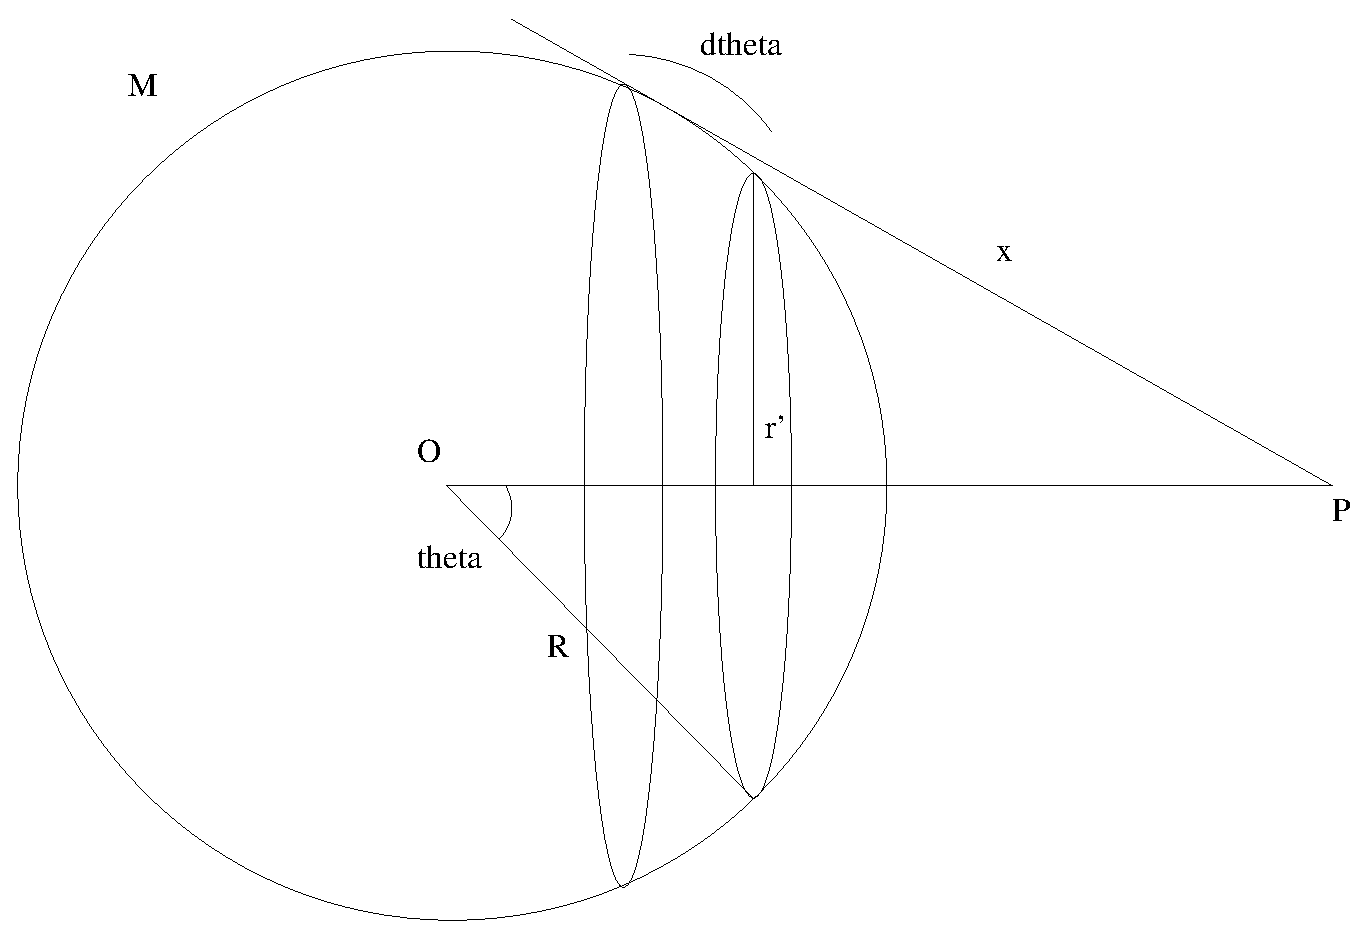
\includegraphics[scale=0.3]{immagini/fisica1/crosta}
\end{figure}
\[F=G\frac{Mm}{r^2}\]
\[r'=R\sin\theta\qquad \ud A=2\pi r'R\ud\theta\]
\[\frac{\ud m}{M}=\frac{\ud
    A}{4\pi R^2}=\frac{2\pi r'R\ud\theta}{4\pi
    R^2}=\frac{R\sin\theta\ud\theta}{2R}=\frac{\sin\theta\ud\theta}{2}\]
\[\ud m=\frac{M\sin\theta\ud\theta}{2}\]
\[U=-\frac{Gmm'}{r}\qquad\ud U=-\frac{G\ud m m'}{x}\]
\[x^2=R^2+r^2-2rR\cos\theta\]
Differenziando si ha:
\[2x\,\ud x=2rR\sin\theta\ud\theta\sin\theta\ud\theta \qquad \sin\theta\ud\theta=\frac{x\ud x}{rR}\]
\begin{align*}
  U & =-\int_{\text{crosta}}\frac{Gm'}{x}\,\ud
  m=-\int_{\text{crosta}}\frac{Gm'}{x}\frac{M\sin\theta\ud\theta}{2}=-\frac{Gm'
  m}{2}\int_{\text{crosta}}\frac{\sin\theta}{x}\ud\theta \\
    & =-\frac{Gmm'}{2rR}\int\frac{x}{x}\ud
  x=-\frac{Gmm'}{2rR}\int_{r-R}^{r+R}\ud
  x=-\frac{Gmm'}{2rR}[r+R-r+R]                           \\
    & =-\frac{Gmm'}{2rR}2R=-\frac{Gmm'}{r}
\end{align*}
Possiamo quindi concentrare tutta la massa nel centro della palla (se $P$ sta fuori).
Se $P$ è esterno:
\[U=-\frac{Gmm'}{r}\qquad F=-\frac{\ud U}{\ud
    r}=\frac{Gmm'}{r^2}\]
Se $P$ è interno vale il discorso precedente fino alla scelta degli
estremi:
\begin{align*}
  U(P) & =-\frac{Gmm'}{2rR}\int_{R-r}^{r+R}\ud x=-\frac{Gmm'}{2rR}[r+R-R+r] \\
       & =-\frac{Gmm'}{2rR}2r=-\frac{Gmm^2}{R}=\const
\end{align*}
\[\ve F=-\frac{\ud U}{\ud \ve r}=0\]

Quindi un punto all'interno del guscio non risente di alcuna
forza, questo lo si può dimostrare ragionando con i coni, in
quanto per ogni cono le forze sono uguali.
\subsection{Caso sfera piena}
All'esterno:
\[F=-G\frac{Mm'}{r^2}\]
Dentro:
\[F=-G\frac{M^{\text{int}}m'}{r^2}\]
\[\frac{M^{\text{int}}}{M^{\text{tot}}}=\frac{V^{\text{int}}}{V^{\text{tot}}}=\frac{\frac{4}{3}\pi r^2\rho}{\frac{4}{3}\pi R^3\rho}\]
\[M^{\text{int}}=\frac{r^3}{R^3}M^{\text{tot}}\]
\[F=-\frac{Gr^3M^{\text{tot}}m'}{r^2R^3}=-\frac{Gmm'r}{R^3}=-kr\]
ha l'espressione di una forza elastica.

\begin{Es}[posta pneumatica interterrestre]
  Immaginiamo di fare un buco che attraversa tutta la terra, passando per il centro. Un pacco lanciato al suo interno sarebbe sottoposto ad una forza del tipo:
  \[F=-kr\qquad k=\left(G\frac{m'M_T}{R_T^3}\right)\]
  \[T=2\pi\sqrt{\frac{m'}{k}}=2\pi\sqrt{\frac{R_T^3}{GM_T}}=2\pi\sqrt{\frac{R_T}{g}}\simeq \SI{40}{\minute} \]
\end{Es}
\section{Interpretazione delle leggi di Keplero}
\subsection{Seconda legge}

L'unica ipotesi che utilizziamo è che la forza sia centrale,
quindi il risultato è estendibile a tutte le forze centrali. Una
forza si dice centrale quando è diretta come la congiungente dei
due punti che interagiscono.

\begin{figure}[htbp]
  \centering
  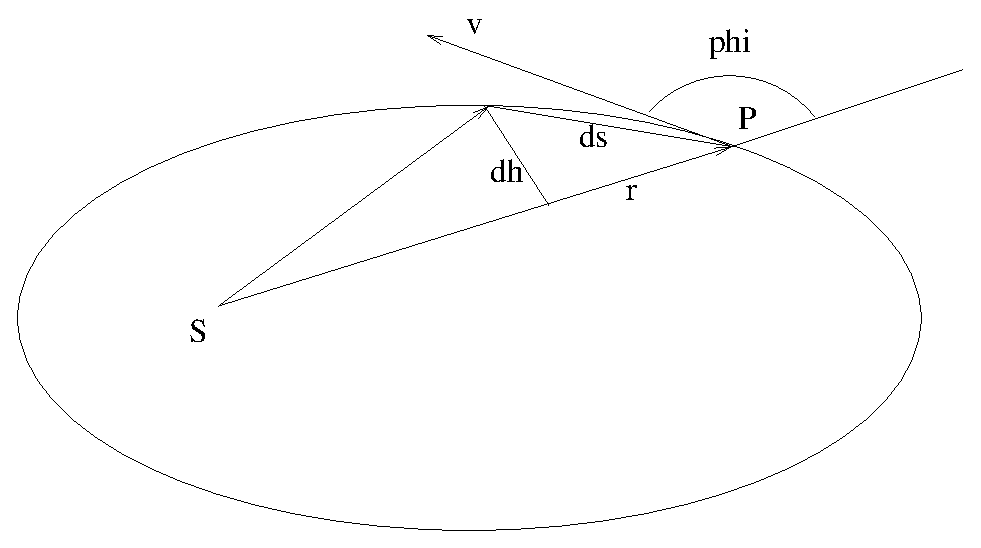
\includegraphics[scale=0.45]{immagini/fisica1/keplero}
\end{figure}



\[
  \frac{\ud\ve L_S}{\ud t}=\ve\tau_S=0\quad\text{perché }\ve
  F\parallel\ve r
\]
\[\ve L_S=\ve r\times m\ve v=\overrightarrow{\const}\]
\[L_S=rmv\sin\phi={\const}\]
\[\ud h=\ud s\sin\phi\]
\index{velocità!areolare}
\[
  \text{velocità areolare}=\frac{\ud A}{\ud t}=\frac{r\ud h}{2\ud
    t}=\frac{r\sin\phi\ud s}{2\ud t}=\frac{r}{2}v\sin\phi
\]
\[L_S=\frac{\ud A}{\ud t}2m\qquad\frac{\ud A}{\ud
    t}=\frac{L_S}{2m}=\const\]
\subsection{Terza legge}
\[F=\frac{GM_Sm}{R^2}=ma=\frac{mv^2}{R}=\omega^2Rm\]
\[\frac{GM_S}{R^2}=\omega^2R\qquad \omega=\frac{2\pi}{T}\]
\[\frac{GM_S}{R^2}=\frac{4\pi^2}{T^2}R\qquad
  T^2=\frac{4\pi^2}{GM_S}R^3\]
\[\frac{T^2}{R^3}=\frac{4\pi^2}{GM_S}=\const\]

\section{\index{accelerazione!di gravità}Accelerazione di gravità}
\begin{Def}{Accelerazione di gravità}
  \[\ve g=\frac{\ve F}{m}\]
  dove $m$ è la massa del corpo su cui viene esercitata la forza.
\end{Def}
Sulla Terra: \[g = \frac{G\frac{M_Tm}{R_T^2}}{m}=\frac{GM_T}{R_T^2}\simeq \SI{9.836}{\meter\per\second\squared} \]
In realtà questo valore è variabile, dall'equatore ai poli, cioè
circa tra $9.78\div9.86$, a causa della forza centrifuga e dallo
schiacciamento dei poli. Per quanto riguarda la forza centrifuga
questa è nulla ai poli e massima all'equatore quindi:
\[F_C=m\omega^2R\qquad F_N=mg_{\text{polo}}\]
\[\frac{F_C}{F_N}=\frac{\omega^2R}{g_{\text{polo}}}=\frac{(2\pi)^2}{T^2}\frac{R}{g_{\text{polo}}}\]
\begin{Es}[Satelliti geostazionari]
  I satelliti geostazionari sono satelliti che per il sistema di riferimento della Terra, sono fermi. Questo vuol dire che hanno lo stesso periodo della Terra:
  \[
    F = G\frac{Mm}{R^2} = m\frac{v^2}{R}\quad\Rightarrow v=\sqrt{\frac{GM}{R}}
  \]
  \[
    T = \frac{2 \pi}{\omega} = \frac{2\pi R}{v} = 2\pi R\sqrt{\frac{R}{GM}} = \SI{1}{\day}
  \]
  \[
    R = \sqrt[3]{\frac{GMT^2}{4\pi^2}}\simeq \SI{42E3}{\kilo\meter}
  \]
  quindi l'altitudine sarà $d = R - R_\oplus\simeq \SI{36E3}{\kilo\meter}$.
\end{Es}

\section{\index{bilancia!di torsione}Misurazione della costante di gra\-vi\-ta\-zio\-ne u\-ni\-ver\-sa\-le}
Cavendish con l'articolo ``Misura della massa terrestre'' nel
1798 è il primo a misurare la costante di gravitazione universale
o costante di Cavendish. Cavendish si proponeva di misurare la
massa terrestre e quindi indirettamente $G$.

La bilancia di torsione viene fatta oscillare, il momento è
proporzionale all'angolo di scostamento dalla posizione di
equilibrio, si genera un moto armonico.

\[\tau=-k\theta=I\alpha\qquad\alpha=\frac{\ud^2\theta}{\ud t^2}\]
\[-k\theta=I\ddot\theta\qquad T=2\pi\sqrt\frac{I}{k}\qquad I=2mD^2\]


Da qui sperimentalmente si trova $k$. Avvicinando delle masse più
grosse si genera un momento dovuto alla forza gravitazionale. Si
impone che il momento gravitazionale sia uguale al momento dovuto
alla forza elastica di richiamo.

\[\tau_\text{Newton}=2\frac{GMm}{d^2}D=\tau_\text{torsione}=k\theta\]
\[G=\frac{k\theta d^2}{2MmD}\]
\section{Massa gravitazione e massa inerziale}
Per massa inerziale si intende quella grandezza usata in dinamica
per esempio \mbox{$\ve F=m\ve a$}. Per massa gravitazionale si intende quella usata nella gravitazione per esempio $F=G\frac{Mm}{r^2}$. Anche se la questione è aperta $m_i$ è proporzionale a $m_g$ infatti se $B$ e $C$ sono attratti da $A$ si ha:
\[\frac{F_{BA}}{F_{CA}}=\frac{Gm_{Bg}m_{ag}}{Gm_{Cg}m_{ag}}=\frac{m_{Bg}}{m_{Cg}}=\frac{m_{Bi}a_b}{m_{ci}a_c}\]
\[\text{se }a_C=a_B\Rightarrow\frac{m_{Bg}}{m_{Cg}}=\frac{m_{Bi}}{m_{Ci}}\Rightarrow
  m_{Bg}=\frac{m_{Cg}}{m_{Ci}}\cdot m_{Bi}\]
\section{\index{principio!di equivalenza}Principio di equivalenza}
\begin{Pri}[equivalenza di Einstein]
  nessun esperimento può rivelare la differenza tra un sistema di riferimento inerziale immerso in un campo gravitazionale $\ve j$ e un sistema non inerziale con accelerazione costante $\ve a=-\ve j$
\end{Pri}
\section{\index{energia!di un'orbita}Energia associata ad un'orbita}
\[E=\frac{1}{2}mv^2-G\frac{Mm}{r^2}=-G\frac{Mm}{2a}\]
\[r(\theta)=\frac{p}{1+e\cos\theta}\]
\[p=\frac{L^2}{m\alpha}\]
\[\alpha=GMm\]
\[e=\text{eccentricità}=\sqrt{1+2^{\frac{EL^2}{m\alpha}}}\]
\[\begin{array}{llc}
    e>1   & E>0 & \text{iperbole}      \\
    e=1   & E=0 & \text{parabola}      \\
    0<e<1 & E<0 & \text{ellisse}       \\
    e=0   & E<0 & \text{circonferenza} \\
  \end{array}\]
